\documentclass[letterpaper,12pt]{article}\usepackage[]{graphicx}\usepackage[]{color}
%% maxwidth is the original width if it is less than linewidth
%% otherwise use linewidth (to make sure the graphics do not exceed the margin)
\makeatletter
\def\maxwidth{ %
  \ifdim\Gin@nat@width>\linewidth
    \linewidth
  \else
    \Gin@nat@width
  \fi
}
\makeatother

\definecolor{fgcolor}{rgb}{0.345, 0.345, 0.345}
\newcommand{\hlnum}[1]{\textcolor[rgb]{0.686,0.059,0.569}{#1}}%
\newcommand{\hlstr}[1]{\textcolor[rgb]{0.192,0.494,0.8}{#1}}%
\newcommand{\hlcom}[1]{\textcolor[rgb]{0.678,0.584,0.686}{\textit{#1}}}%
\newcommand{\hlopt}[1]{\textcolor[rgb]{0,0,0}{#1}}%
\newcommand{\hlstd}[1]{\textcolor[rgb]{0.345,0.345,0.345}{#1}}%
\newcommand{\hlkwa}[1]{\textcolor[rgb]{0.161,0.373,0.58}{\textbf{#1}}}%
\newcommand{\hlkwb}[1]{\textcolor[rgb]{0.69,0.353,0.396}{#1}}%
\newcommand{\hlkwc}[1]{\textcolor[rgb]{0.333,0.667,0.333}{#1}}%
\newcommand{\hlkwd}[1]{\textcolor[rgb]{0.737,0.353,0.396}{\textbf{#1}}}%
\let\hlipl\hlkwb

\usepackage{framed}
\makeatletter
\newenvironment{kframe}{%
 \def\at@end@of@kframe{}%
 \ifinner\ifhmode%
  \def\at@end@of@kframe{\end{minipage}}%
  \begin{minipage}{\columnwidth}%
 \fi\fi%
 \def\FrameCommand##1{\hskip\@totalleftmargin \hskip-\fboxsep
 \colorbox{shadecolor}{##1}\hskip-\fboxsep
     % There is no \\@totalrightmargin, so:
     \hskip-\linewidth \hskip-\@totalleftmargin \hskip\columnwidth}%
 \MakeFramed {\advance\hsize-\width
   \@totalleftmargin\z@ \linewidth\hsize
   \@setminipage}}%
 {\par\unskip\endMakeFramed%
 \at@end@of@kframe}
\makeatother

\definecolor{shadecolor}{rgb}{.97, .97, .97}
\definecolor{messagecolor}{rgb}{0, 0, 0}
\definecolor{warningcolor}{rgb}{1, 0, 1}
\definecolor{errorcolor}{rgb}{1, 0, 0}
\newenvironment{knitrout}{}{} % an empty environment to be redefined in TeX

\usepackage{alltt}
\usepackage[top=1in,bottom=1in,left=1in,right=1in]{geometry}
\usepackage{setspace}
\usepackage[colorlinks=true,urlcolor=blue,citecolor=blue,linkcolor=blue]{hyperref}
\usepackage{indentfirst}
\usepackage{multirow}
\usepackage{booktabs}
\usepackage[final]{animate}
\usepackage{graphicx}
\usepackage{verbatim}
\usepackage{rotating}
\usepackage{tabularx}
\usepackage{array}
\usepackage{subfig} 
\usepackage[noae]{Sweave}
\usepackage{cleveref}
\usepackage[figureposition=bottom]{caption}
\usepackage{paralist}
\usepackage{acronym}
\usepackage{outlines}
\usepackage{pdflscape}

%for supplemental figures/tables
\newcommand{\beginsupplement}{%
        \setcounter{table}{0}
        \renewcommand{\thetable}{S\arabic{table}}%
        \setcounter{figure}{0}
        \renewcommand{\thefigure}{S\arabic{figure}}%
     }

% knitr options




\IfFileExists{upquote.sty}{\usepackage{upquote}}{}
\begin{document}

%%%%%%
% figures 

\setcounter{figure}{1}
% \setcounter{table}{1}

\begin{landscape}
\centering\vspace*{\fill}
\begin{figure}[!ht]

{\centering 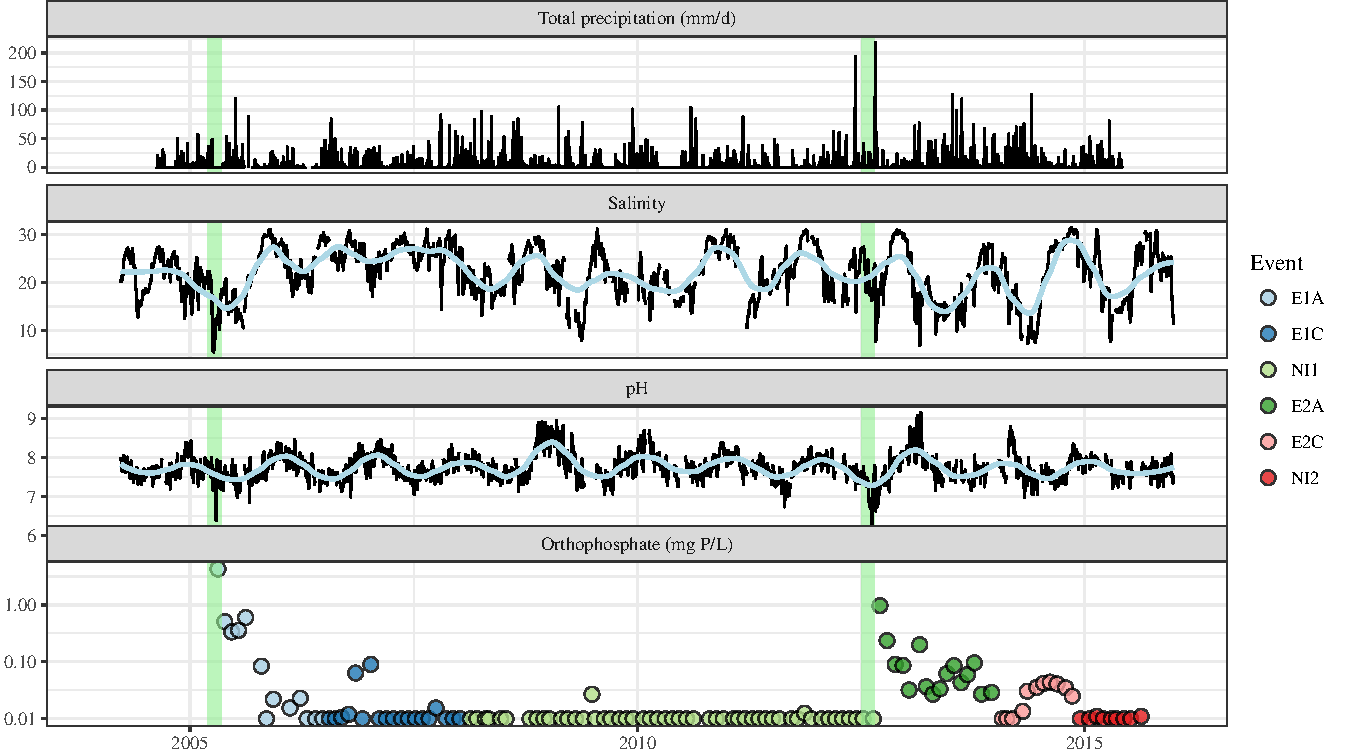
\includegraphics[width=1.3\textwidth]{figs/Fig2} 

}

\caption[Time series of total precipitation, salinity, pH, and phosphate for Bangs Lake, Grand Bay reserve]{Time series of total precipitation, salinity, pH, and phosphate for Bangs Lake, Grand Bay reserve.  All observations are daily averages, excluding phosphate which was sampled monthly.  Vertical green bars indicate a heavy rain event in April 2005 and hurricane Isaac in August 2012.  Salinity and pH include a loess smooth to reduce variability. Orthophosphate is colored by event categories in relation to the vertical green bars.  E1A: event 1 acute, E1C: event 1 chronic, NI1: non-impact 1, E2A: event 2 acute, E2C: event 2 chronic, and NI2: non-impact 2.}\label{fig:Fig2}
\end{figure}


\end{landscape}
\clearpage

\begin{figure}[!ht]

{\centering 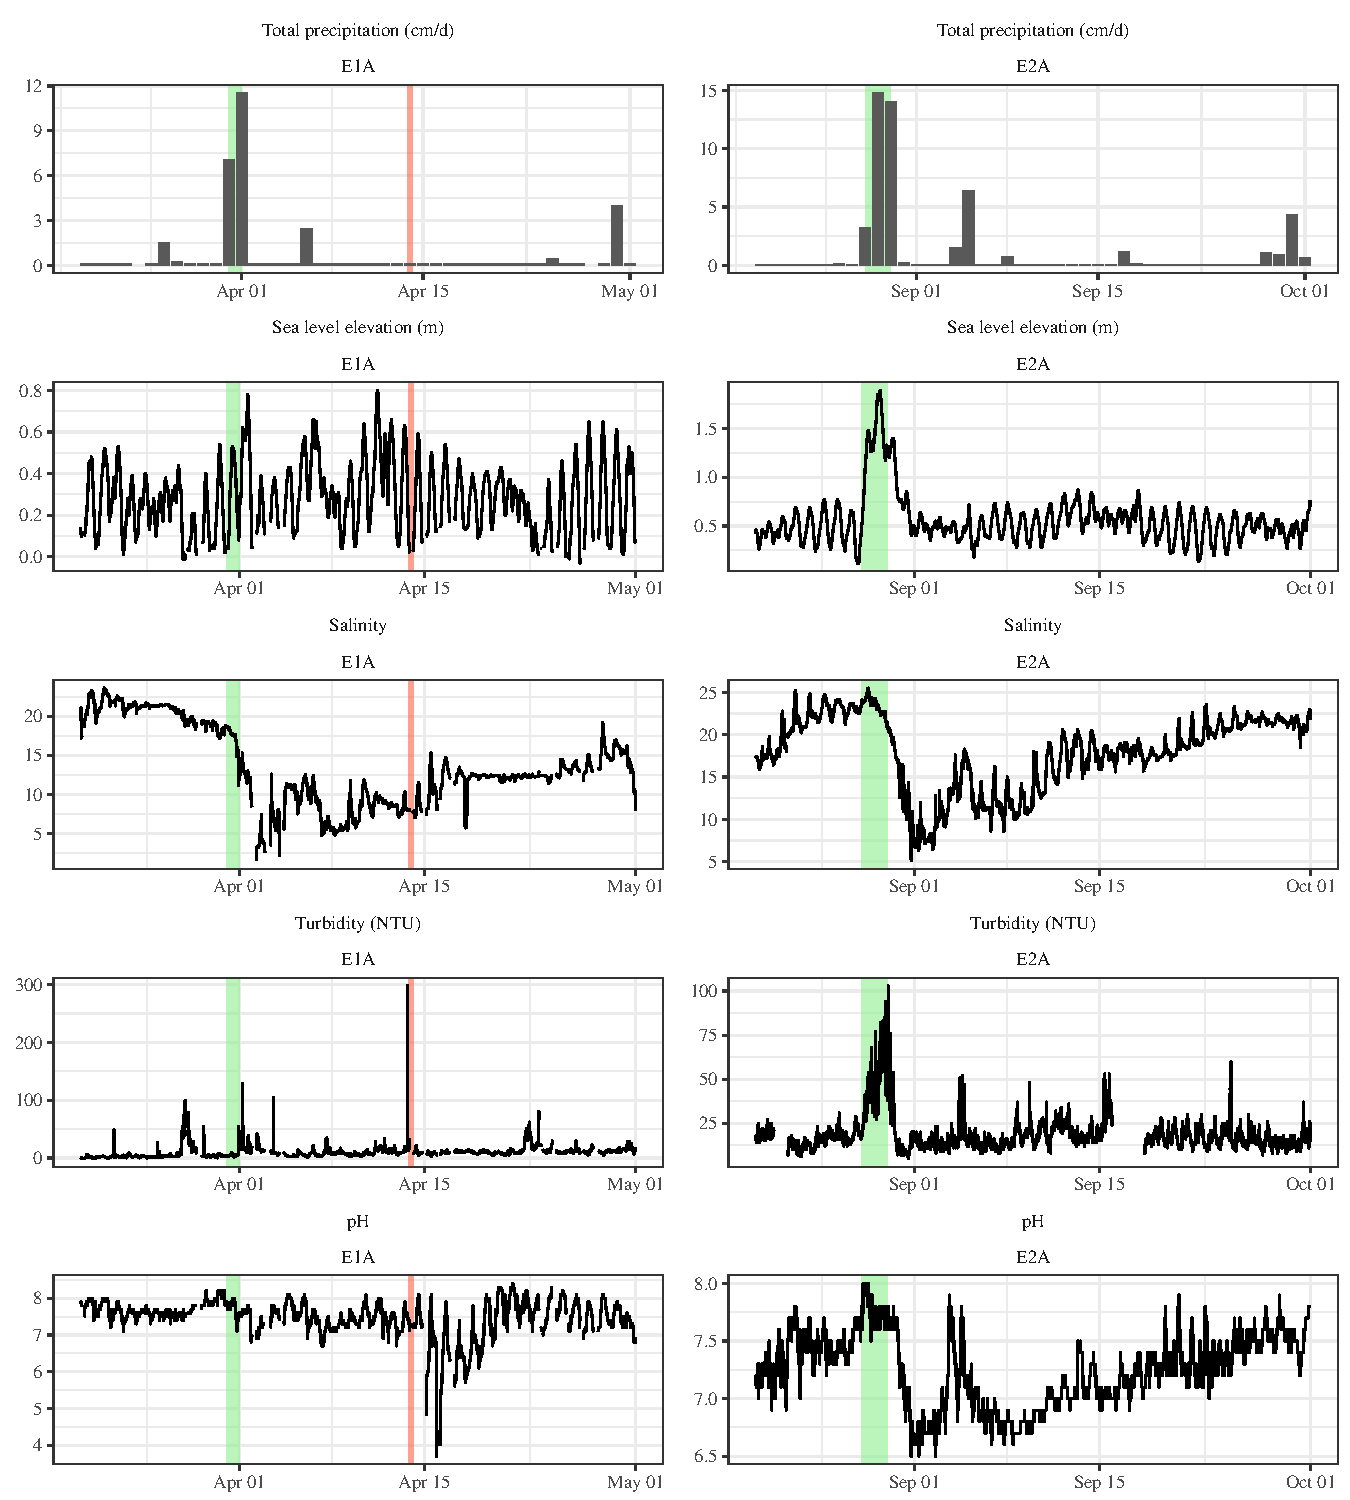
\includegraphics[width=\maxwidth]{figs/Fig3} 

}

\caption[Time series of daily precipitation, sea level elevation, salinity, turbidity, and pH for Bangs Lake, Grand Bay reserve]{Time series of daily precipitation, sea level elevation, salinity, turbidity, and pH for Bangs Lake, Grand Bay reserve.  Precipitation data are daily totals from the Pascagoula International Airport.  All other data were collected at 15 minute time steps.  Green shading indicates period of high precipitation for a heavy rain event in 2005 (left, March 31\textsuperscript{st} to April 1\textsuperscript{st}) and hurricane Isaac in 2012 (right, August 28\textsuperscript{th} to 30\textsuperscript{th}).  Red shading for the first event indicates the date of documented phosphorus spill.  E1A: event 1 acute, E2A: event 2 acute.}\label{fig:Fig3}
\end{figure}


\clearpage

\begin{figure}[!ht]

{\centering 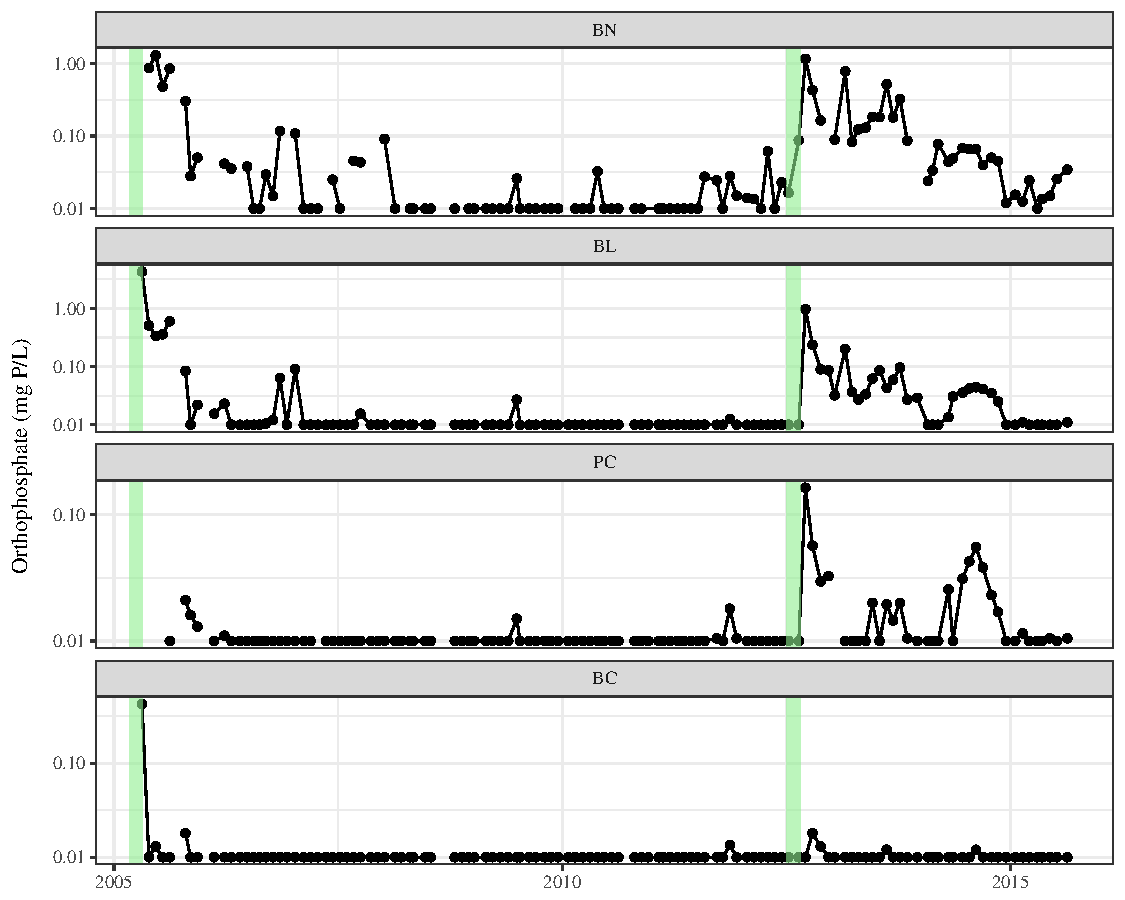
\includegraphics[width=\maxwidth]{figs/Fig4} 

}

\caption[Monthly phosphate time series at Bangs North (BN), Bangs Lake (BL), Point aux Chenes (PC), and Bayou Cumbest (BC) sites at Grand Bay]{Monthly phosphate time series at Bangs North (BN), Bangs Lake (BL), Point aux Chenes (PC), and Bayou Cumbest (BC) sites at Grand Bay. Vertical green bars indicate a heavy rain event in April 2005 and hurricane Isaac in August 2012.}\label{fig:Fig4}
\end{figure}


\clearpage

\begin{figure}[!ht]

{\centering 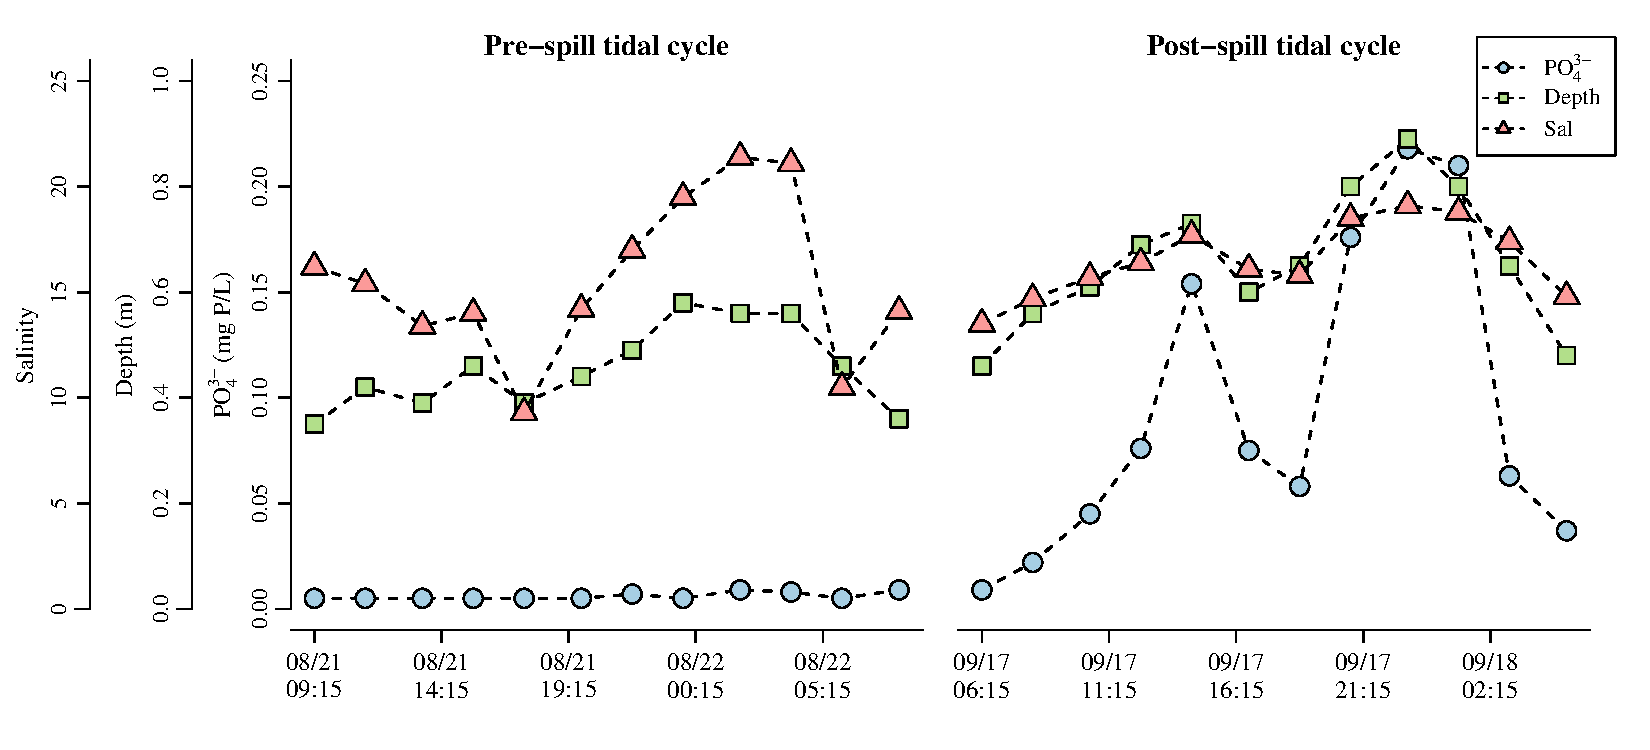
\includegraphics[width=\maxwidth]{figs/Fig5} 

}

\caption[Diel phosphate and salinity data before and after Hurricane Isaac during the second spill event]{Diel phosphate and salinity data before and after Hurricane Isaac during the second spill event. Bayou Cumbest, is approximately 7 km (hydrologically) from the spill site and elevated phosphorus is observed with tidal influx (depth) following the event.}\label{fig:Fig5}
\end{figure}



\begin{figure}[!ht]

{\centering 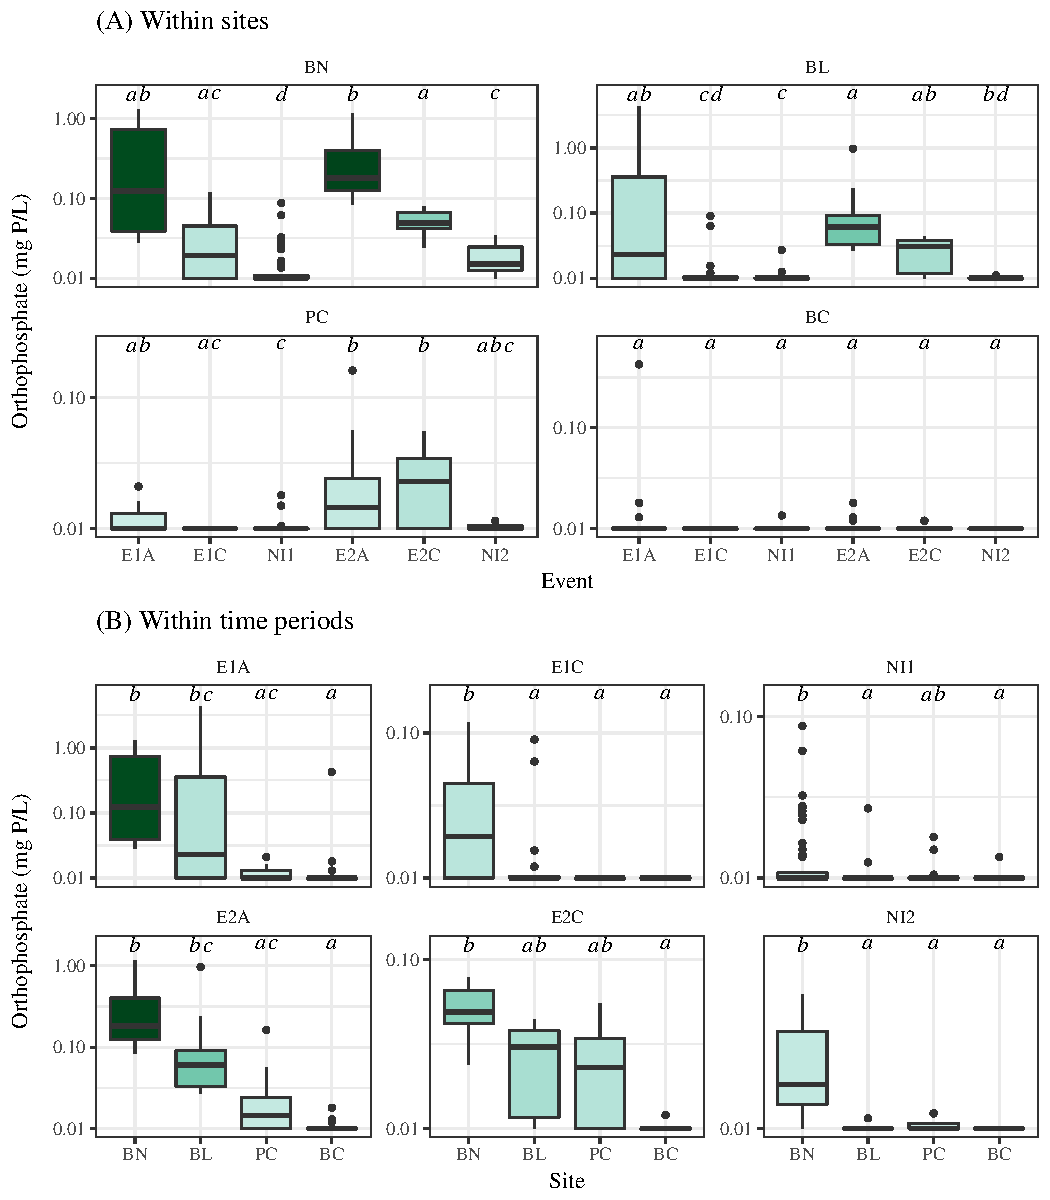
\includegraphics[width=\maxwidth]{figs/Fig6} 

}

\caption[Boxplot summaries of monthly orthophosphate data for (A) time frames group by site and (B) sites grouped by time frame]{Boxplot summaries of monthly orthophosphate data for (A) time frames group by site and (B) sites grouped by time frame. Boxplots within each panel that do not share a letter have significantly different concentrations. Sites are Bangs Lake (BL), Bangs North (BN), and Point aux Chenes (PC), and Bayou Cumbest (BC).  Time frames are event 1 acute (E1A), event 1 chronic (E1C), non-impact 1 (NI1), event 2 acute (E2A), event 2 chronic (E2C), and non-impact 2 (NI2).}\label{fig:Fig6}
\end{figure}





{\centering 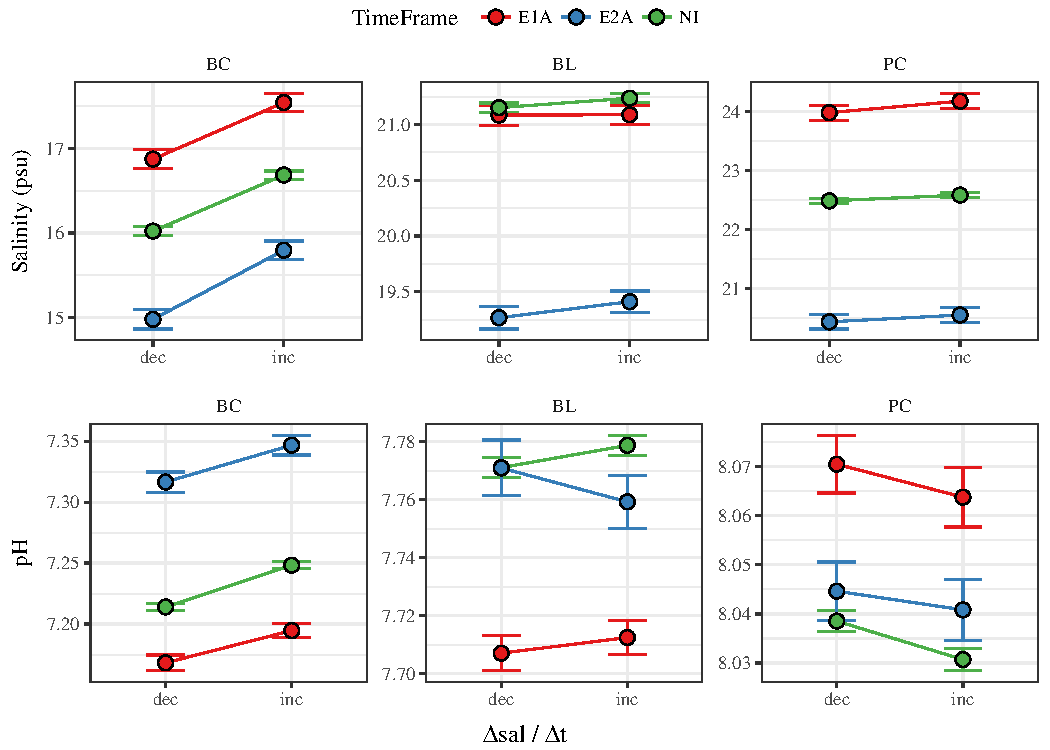
\includegraphics[width=\maxwidth]{figs/Fig7} 

}




\clearpage

%%%%%%
% tables

% summary charactistics table
%latex.default(tab, file = "", rowlabel = "Stations", caption = cap,     caption.loc = "top", rgroup = rgrps, n.rgroup = rep(4, 7),     rowname = rows, colheads = c("Average", "Median", "St. Dev",         "Min", "Max"), label = "tab:summtab")%
\begin{table}[!tbp]
\caption{Site summaries of water quality (hourly) and nutrient (monthly) observations from 2005 to 2015.  Units are mg L$^{-1}$ for all variables, except Chl-\textit{a} as $\mu$g L$^{-1}$, DO\textit{sat} as percent, pH from 0-12, and salinity as psu. Nutrient summaries are based on maximum likelihood estimates for left-censored data.  Sites are BC: Bayou Cumbest, BH: Bayou Heron (no nutrient data), BL: Bangs Lake, BN: Bangs North (no water quality data), and PC: Point aux Chenes.\label{tab:summtab}} 
\begin{center}
\begin{tabular}{lrrrrr}
\hline\hline
\multicolumn{1}{l}{Stations}&\multicolumn{1}{c}{Average}&\multicolumn{1}{c}{Median}&\multicolumn{1}{c}{St. Dev}&\multicolumn{1}{c}{Min}&\multicolumn{1}{c}{Max}\tabularnewline
\hline
{\bfseries Chl-\textit{a}}&&&&&\tabularnewline
~~BN&$ 7.94$&$ 5.01$&$ 9.79$&$0.55$&$ 36.71$\tabularnewline
~~BL&$ 8.25$&$ 5.43$&$ 9.44$&$0.46$&$ 41.98$\tabularnewline
~~PC&$ 7.98$&$ 5.17$&$ 9.39$&$0.52$&$ 33.95$\tabularnewline
~~BC&$10.82$&$ 6.69$&$13.76$&$0.69$&$ 47.67$\tabularnewline
\hline
{\bfseries DO$_{sat}$}&&&&&\tabularnewline
~~BL&$92.05$&$93.10$&$16.26$&$8.60$&$297.70$\tabularnewline
~~PC&$97.08$&$97.90$&$15.52$&$8.40$&$221.90$\tabularnewline
~~BC&$80.12$&$80.90$&$19.11$&$1.80$&$221.90$\tabularnewline
~~BH&$45.26$&$47.00$&$27.19$&$0.00$&$165.80$\tabularnewline
\hline
{\bfseries NH$_4^+$}&&&&&\tabularnewline
~~BN&$ 0.03$&$ 0.01$&$ 0.07$&$0.01$&$  0.16$\tabularnewline
~~BL&$ 0.02$&$ 0.01$&$ 0.06$&$0.01$&$  0.18$\tabularnewline
~~PC&$ 0.02$&$ 0.01$&$ 0.06$&$0.01$&$  0.42$\tabularnewline
~~BC&$ 0.04$&$ 0.01$&$ 0.08$&$0.01$&$  0.21$\tabularnewline
\hline
{\bfseries NO$_2^-$/NO$_3^{2-}$}&&&&&\tabularnewline
~~BN&$ 0.01$&$ 0.00$&$ 0.02$&$0.01$&$  0.10$\tabularnewline
~~BL&$ 0.01$&$ 0.00$&$ 0.03$&$0.01$&$  0.09$\tabularnewline
~~PC&$ 0.01$&$ 0.00$&$ 0.04$&$0.01$&$  0.10$\tabularnewline
~~BC&$ 0.01$&$ 0.01$&$ 0.02$&$0.01$&$  0.09$\tabularnewline
\hline
{\bfseries pH}&&&&&\tabularnewline
~~BL&$ 7.75$&$ 7.70$&$ 0.37$&$3.70$&$  9.60$\tabularnewline
~~PC&$ 8.06$&$ 8.10$&$ 0.22$&$7.00$&$  9.00$\tabularnewline
~~BC&$ 7.26$&$ 7.30$&$ 0.46$&$5.10$&$  9.00$\tabularnewline
~~BH&$ 6.88$&$ 7.00$&$ 0.64$&$4.00$&$  8.40$\tabularnewline
\hline
{\bfseries PO$_4^{3-}$}&&&&&\tabularnewline
~~BN&$ 0.12$&$ 0.02$&$ 0.90$&$0.01$&$  1.29$\tabularnewline
~~BL&$ 0.09$&$ 0.00$&$ 2.13$&$0.01$&$  4.29$\tabularnewline
~~PC&$ 0.01$&$ 0.00$&$ 0.02$&$0.01$&$  0.16$\tabularnewline
~~BC&$ 0.00$&$ 0.00$&$ 0.03$&$0.01$&$  0.43$\tabularnewline
\hline
{\bfseries Salinity}&&&&&\tabularnewline
~~BL&$22.02$&$22.40$&$ 5.49$&$1.50$&$ 32.10$\tabularnewline
~~PC&$23.30$&$24.30$&$ 5.37$&$4.30$&$ 33.20$\tabularnewline
~~BC&$17.22$&$18.00$&$ 7.86$&$0.00$&$ 33.50$\tabularnewline
~~BH&$17.93$&$19.50$&$ 7.50$&$0.00$&$ 32.40$\tabularnewline
\hline
\end{tabular}\end{center}
\end{table}

\clearpage

% kendall tests
%latex.default(tab, file = "", rowlabel = "", caption = cap, caption.loc = "top",     rgroup = rgrp, n.rgroup = nrgrp, rowname = rows, colheads = c("$\\tau$",         "slope", "median", "\\% change"), label = paste0("tab:",         nut, "trnd"))%
\begin{table}[!tbp]
\caption{Summary of orthophosphate (mg P/L) trends for time periods with sufficient data.  Trends are based on seasonal Kendall tests, where $\tau$ is the direction and strength of the trend, slope is the change per year, median is the median in the time period, and percent change is the slope divided by the median.\label{tab:PO4Ftrnd}} 
\begin{center}
\begin{tabular}{lllll}
\hline\hline
\multicolumn{1}{l}{}&\multicolumn{1}{c}{$\tau$}&\multicolumn{1}{c}{slope}&\multicolumn{1}{c}{median}&\multicolumn{1}{c}{\% change}\tabularnewline
\hline
{\bfseries E1A, E1C}&&&&\tabularnewline
~~BN&-0.48&-0.03&0.04&-79.25\tabularnewline
~~BL&-0.66**&-0.02&0.01&-236.25\tabularnewline
~~PC&-0.31*&0.00&0.01&0.00\tabularnewline
~~BC&-0.19&0.00&0.01&0.00\tabularnewline
\hline
{\bfseries NI1}&&&&\tabularnewline
~~BN&0.37**&0.00&0.01&0.00\tabularnewline
~~BL&0.02&0.00&0.01&0.00\tabularnewline
~~PC&0.10&0.00&0.01&0.00\tabularnewline
~~BC&0.04&0.00&0.01&0.00\tabularnewline
\hline
{\bfseries E2A, E2C}&&&&\tabularnewline
~~BN&-1.00**&-0.12&0.09&-134.88\tabularnewline
~~BL&-0.85**&-0.04&0.04&-104.79\tabularnewline
~~PC&0.12&0.00&0.02&0.00\tabularnewline
~~BC&-0.15&0.00&0.01&0.00\tabularnewline
\hline
\end{tabular}\end{center}
\end{table}
%latex.default(tab, file = "", rowlabel = "", caption = cap, caption.loc = "top",     rgroup = rgrp, n.rgroup = nrgrp, rowname = rows, colheads = c("$\\tau$",         "slope", "median", "\\% change"), label = paste0("tab:",         nut, "trnd"))%
\begin{table}[!tbp]
\caption{Summary of ammonium (mg N/L) trends for time periods with sufficient data.  Trends are based on seasonal Kendall tests, where $\tau$ is the direction and strength of the trend, slope is the change per year, median is the median in the time period, and percent change is the slope divided by the median.\label{tab:NH4Ftrnd}} 
\begin{center}
\begin{tabular}{lllll}
\hline\hline
\multicolumn{1}{l}{}&\multicolumn{1}{c}{$\tau$}&\multicolumn{1}{c}{slope}&\multicolumn{1}{c}{median}&\multicolumn{1}{c}{\% change}\tabularnewline
\hline
{\bfseries E1A, E1C}&&&&\tabularnewline
~~BN&-0.12&-0.01&0.03&-26.03\tabularnewline
~~BL&-0.20&-0.01&0.03&-41.73\tabularnewline
~~PC&-0.17&-0.01&0.03&-18.46\tabularnewline
~~BC&-0.07&0.00&0.03&-5.13\tabularnewline
\hline
{\bfseries NI1}&&&&\tabularnewline
~~BN&0.13&0.00&0.02&19.35\tabularnewline
~~BL&-0.19&0.00&0.01&0.00\tabularnewline
~~PC&-0.18&0.00&0.01&0.00\tabularnewline
~~BC&0.00&0.00&0.02&0.00\tabularnewline
\hline
{\bfseries E2A, E2C}&&&&\tabularnewline
~~BN&-0.32&0.00&0.01&-4.55\tabularnewline
~~BL&-0.04&0.00&0.01&0.00\tabularnewline
~~PC&-0.22&0.00&0.01&0.00\tabularnewline
~~BC&-0.30&0.00&0.01&-11.25\tabularnewline
\hline
\end{tabular}\end{center}
\end{table}
%latex.default(tab, file = "", rowlabel = "", caption = cap, caption.loc = "top",     rgroup = rgrp, n.rgroup = nrgrp, rowname = rows, colheads = c("$\\tau$",         "slope", "median", "\\% change"), label = paste0("tab:",         nut, "trnd"))%
\begin{table}[!tbp]
\caption{Summary of nitrite/nitrate (mg N/L) trends for time periods with sufficient data.  Trends are based on seasonal Kendall tests, where $\tau$ is the direction and strength of the trend, slope is the change per year, median is the median in the time period, and percent change is the slope divided by the median.\label{tab:NO23Ftrnd}} 
\begin{center}
\begin{tabular}{lllll}
\hline\hline
\multicolumn{1}{l}{}&\multicolumn{1}{c}{$\tau$}&\multicolumn{1}{c}{slope}&\multicolumn{1}{c}{median}&\multicolumn{1}{c}{\% change}\tabularnewline
\hline
{\bfseries E1A, E1C}&&&&\tabularnewline
~~BN&0.08&0.00&0.01&0.00\tabularnewline
~~BL&-0.21&0.00&0.01&0.00\tabularnewline
~~PC&-0.48*&0.00&0.01&0.00\tabularnewline
~~BC&-0.18&0.00&0.01&0.00\tabularnewline
\hline
{\bfseries NI1}&&&&\tabularnewline
~~BN&-0.09&0.00&0.01&0.00\tabularnewline
~~BL&-0.10&0.00&0.01&0.00\tabularnewline
~~PC&-0.08&0.00&0.01&0.00\tabularnewline
~~BC&-0.11&0.00&0.01&0.00\tabularnewline
\hline
{\bfseries E2A, E2C}&&&&\tabularnewline
~~BN&-0.09&0.00&0.01&0.00\tabularnewline
~~BL&-0.08&0.00&0.01&0.00\tabularnewline
~~PC&-0.08&0.00&0.01&0.00\tabularnewline
~~BC&0.00&0.00&0.01&0.00\tabularnewline
\hline
\end{tabular}\end{center}
\end{table}
%latex.default(tab, file = "", rowlabel = "", caption = cap, caption.loc = "top",     rgroup = rgrp, n.rgroup = nrgrp, rowname = rows, colheads = c("$\\tau$",         "slope", "median", "\\% change"), label = paste0("tab:",         nut, "trnd"))%
\begin{table}[!tbp]
\caption{Summary of chlorophyll-a ($\mu$g/L) trends for time periods with sufficient data.  Trends are based on seasonal Kendall tests, where $\tau$ is the direction and strength of the trend, slope is the change per year, median is the median in the time period, and percent change is the slope divided by the median.\label{tab:CHLA_Ntrnd}} 
\begin{center}
\begin{tabular}{lllll}
\hline\hline
\multicolumn{1}{l}{}&\multicolumn{1}{c}{$\tau$}&\multicolumn{1}{c}{slope}&\multicolumn{1}{c}{median}&\multicolumn{1}{c}{\% change}\tabularnewline
\hline
{\bfseries NI1}&&&&\tabularnewline
~~BN&0.61**&2.24&3.98&56.36\tabularnewline
~~BL&0.67**&2.14&4.66&45.98\tabularnewline
~~PC&0.59**&2.12&6.63&31.90\tabularnewline
~~BC&0.39**&2.17&6.34&34.29\tabularnewline
\hline
{\bfseries E2A, E2C}&&&&\tabularnewline
~~BN&0.36&1.21&6.12&19.69\tabularnewline
~~BL&0.56&1.25&6.86&18.23\tabularnewline
~~PC&-0.04&0.01&5.96&0.13\tabularnewline
~~BC&0.26&1.42&6.92&20.52\tabularnewline
\hline
\end{tabular}\end{center}
\end{table}

\clearpage

% supplements
\beginsupplement

\begin{figure}[!ht]

{\centering 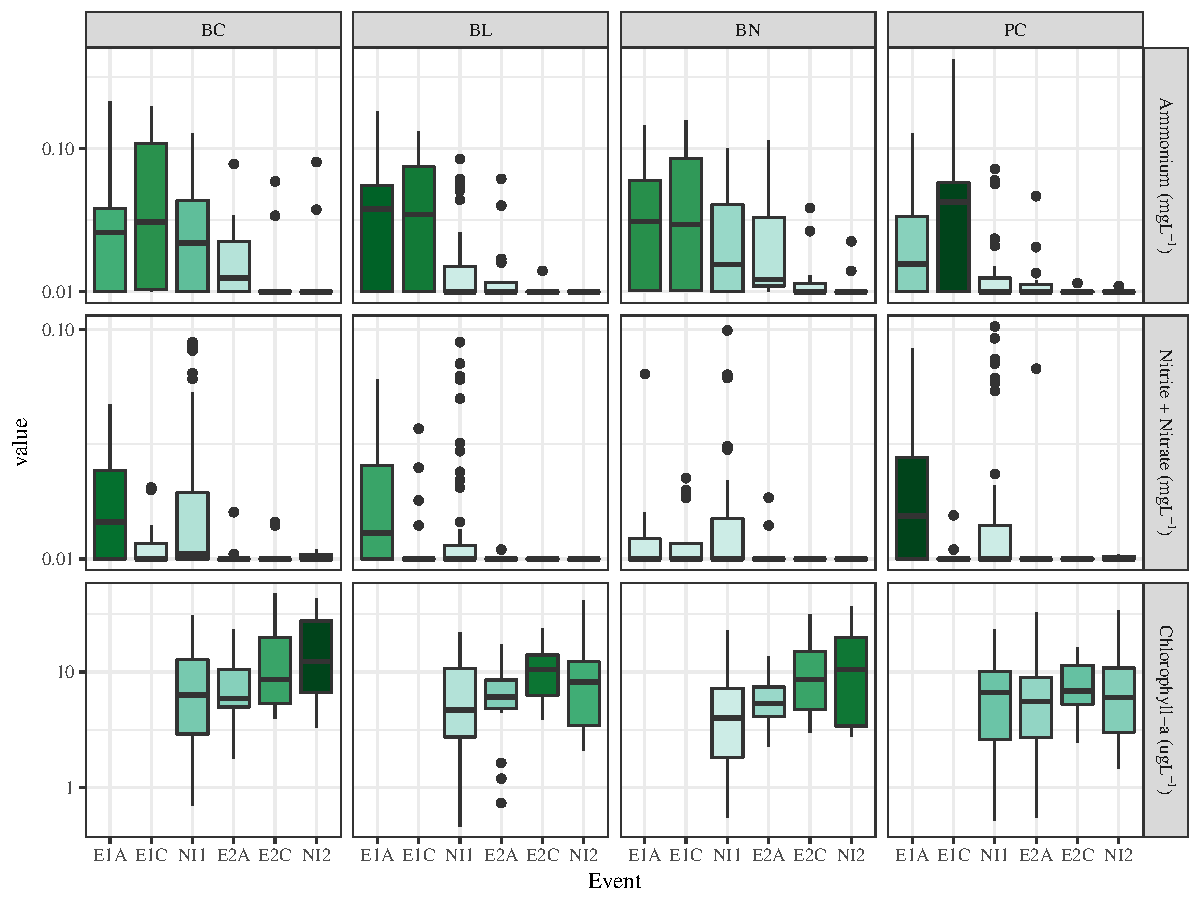
\includegraphics[width=\maxwidth]{figs/FigS1} 

}

\caption[Boxplot summaries of nutrient data for time frames grouped by site]{Boxplot summaries of nutrient data for time frames grouped by site. Boxplots within each panel that do not share a letter have significantly different concentrations. Insufficient chlorophyll data were removed for E1A and E1C. Sites are Bangs Lake (BL), Bangs North (BN), and Point aux Chenes (PC), and Bayou Cumbest (BC).  Time frames are event 1 acute (E1A), event 1 chronic (E1C), non-impact 1 (NI1), event 2 acute (E2A), event 2 chronic (E2C), and non-impact 2 (NI2).}\label{fig:FigS1}
\end{figure}


\clearpage

\begin{figure}[!ht]

{\centering 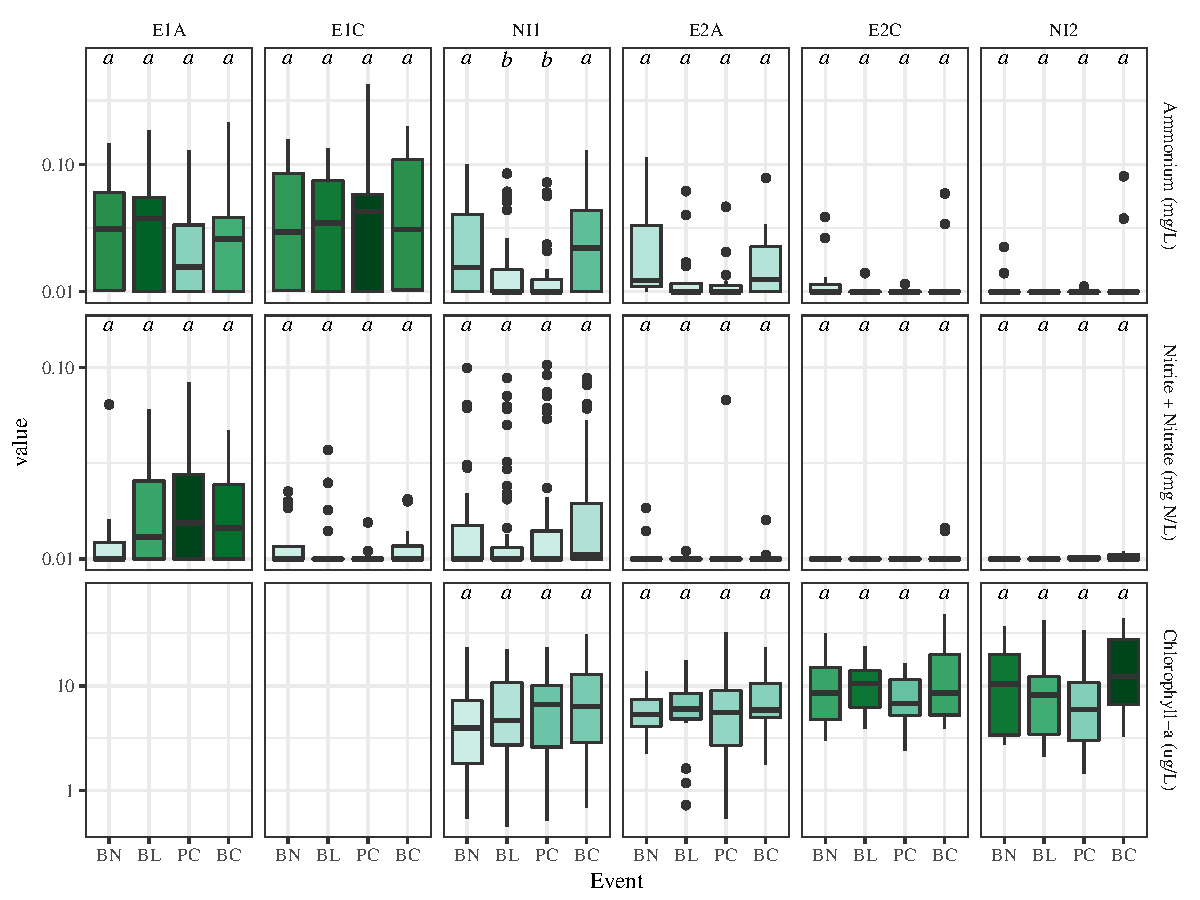
\includegraphics[width=\maxwidth]{figs/FigS2} 

}

\caption[Boxplot summaries of nutrient data for sitres grouped by time frames]{Boxplot summaries of nutrient data for sitres grouped by time frames. Boxplots within each panel that do not share a letter have significantly different concentrations. Insufficient chlorophyll data were removed for E1A and E1C. Sites are Bangs Lake (BL), Bangs North (BN), and Point aux Chenes (PC), and Bayou Cumbest (BC).  Time frames are event 1 acute (E1A), event 1 chronic (E1C), non-impact 1 (NI1), event 2 acute (E2A), event 2 chronic (E2C), and non-impact 2 (NI2).}\label{fig:FigS2}
\end{figure}



\end{document}
